\documentclass[12pt,letterpaper,final]{article}

%\documentstyle[12pt,graphicx,natbib,hyperref,Sweave,rotating]{article}

\usepackage{Sweave}
\usepackage{graphicx}
\usepackage{natbib}
\usepackage{hyperref}
\usepackage{caption}
\usepackage{rotating}
\usepackage{verbatim}
\usepackage{textcomp}

\setlength{\oddsidemargin}{0in}
\setlength{\textwidth}{6.15in}
\setlength{\topmargin}{0.5in}
\setlength{\textheight}{22cm}
\setlength{\headheight}{0in}
\setlength{\headsep}{0in}
\setlength{\parskip}{5pt plus 2pt minus 3pt}

\marginparwidth2cm
\marginparsep0.2cm
\marginparpush0.2cm
%\tabcolsep0pt

\def\thefootnote{\fnsymbol{footnote}}
\setcounter{footnote}{1}

\renewcommand{\baselinestretch}{1.2}
\renewcommand{\labelenumi}{(\roman{enumi})}

\renewcommand{\topfraction}{1.0}
\renewcommand{\bottomfraction}{1.0}
\renewcommand{\textfraction}{0.0}
\renewcommand{\floatpagefraction}{1.0}

\newtheorem{definition}{Definition}
\newtheorem{theorem}{Theorem}
\newtheorem{lemma}[theorem]{Lemma}
\newtheorem{claim}[theorem]{Claim}
\newtheorem{fact}[theorem]{Fact}

% to get nice proofs ...
\newcommand{\qedsymb}{\mbox{ }~\hfill~{\rule{2mm}{2mm}}}
\newenvironment{proof}{\begin{trivlist}
\item[\hspace{\labelsep}{\bf\noindent Proof: }]
}{\qedsymb\end{trivlist}}

\def\printindex{\input{\jobname.ind}}

\newfont{\msymb}{cmsy10 scaled 1000}

\def\nullset{\mbox{\O}}
\def\R{{I\!\!R}}
\def\N{{I\!\!N}}
\def\C{{C\!\!\!\!I}}

\def\convdist{\stackrel{d}{\longrightarrow}}
\def\convlaw{\stackrel{L}{\longrightarrow}}
\def\convweak{\stackrel{w}{\longrightarrow}}
\def\convprob{\stackrel{p}{\longrightarrow}}
\def\convmean#1{\stackrel{#1}{\longrightarrow}}
\def\convas{\stackrel{a.s.}{\longrightarrow}}
\def\convwp{\stackrel{w.p.1}{\longrightarrow}}

\def\A{\mbox{\msymb A}}
\def\B{\mbox{\msymb B}}
\def\H{\mbox{\msymb H}}
\def\P{\mbox{\msymb P}}
\def\S{\mbox{\msymb S}}
\def\X{\mbox{\msymb X}}
\def\Y{\mbox{\msymb Y}}

\def\u0{\underline{0}}
\def\ua{\underline{a}}
\def\ub{\underline{b}}
\def\ud{\underline{d}}
\def\ug{\underline{g}}
\def\ueta{\underline{\eta}}
\def\umu{\underline{\mu}}
\def\utheta{\underline{\theta}}
\def\uvartheta{\underline{\vartheta}}
\def\UT{\underline{T}}
\def\ut{\underline{t}}
\def\UU{\underline{U}}
\def\uu{\underline{u}}
\def\OX{\overline{X}}
\def\UX{\underline{X}}
\def\ux{\underline{x}}
\def\UY{\underline{Y}}
\def\uy{\underline{y}}
\def\UZ{\underline{Z}}
\def\uz{\underline{z}}

%\parskip 0.1in
\pagenumbering{arabic}    %  Start using 1,2,... as page numbers.
\pagestyle{plain}         %  Page numbers in middle bottom of page.
%\setcounter{page}{80}  % XXXXXXXXXXXXXXXXX
%\setcounter{theorem}{5} % XXXXXXXXXXXXXXXXX
%\setcounter{definition}{10} % XXXXXXXXXXXXXXXXX

\parindent 0in

\makeindex


\begin{document}

\Sconcordance{concordance:lect_main.tex:lect_main.Rnw:%
1 164 1}
\Sconcordance{concordance:lect_main.tex:./lect_acknow.Rnw:ofs 165:%
1 40 1}
\Sconcordance{concordance:lect_main.tex:lect_main.Rnw:ofs 206:%
167 13 1}
\Sconcordance{concordance:lect_main.tex:./lect_chapter6.Rnw:ofs 220:%
1 27 1 1 2 12 0 3 1 2 2 1 3 1 0 1 3 1 0 1 1 1 3 1 0 1 1 1 3 1 0 1 1 4 0 %
1 2 6 1 1 2 1 0 1 1 1 3 1 0 1 4 2 0 1 4 2 0 1 5 3 0 1 2 4 0 1 2 15 1 1 %
2 1 0 2 2 1 1 1 2 1 0 1 2 1 1 1 2 1 0 1 2 1 1 1 2 1 0 1 2 1 1 1 2 1 0 1 %
2 1 1 1 2 1 0 1 2 1 1 1 2 5 0 1 2 10 1 1 2 1 0 1 3 1 0 1 1 1 2 1 3 1 0 %
1 1 1 3 1 0 1 1 1 3 1 0 1 1 4 0 1 2 1 1 1 2 1 0 1 1 1 2 1 8 6 0 1 8 6 0 %
1 1 3 0 1 2 1 1 1 9 8 0 1 1 3 0 1 2 1 1 1 7 6 0 1 1 3 0 1 2 1 1 1 2 5 0 %
1 2 21 1 1 2 1 0 1 1 1 2 4 0 2 2 5 0 2 2 5 0 2 2 5 0 2 2 5 0 2 2 5 0 1 %
2 3 1 1 2 1 0 1 1 1 5 3 0 1 1 3 0 1 2 1 1 1 5 4 0 1 1 3 0 1 2 1 1 1 2 5 %
0 1 2 11 1 1 47 49 0 1 2 8 1 1 2 1 0 1 1 1 2 5 0 1 2 5 0 1 2 6 0 1 2 5 %
1 4 0 1 3 5 1 1 2 6 0 1 2 1 4 6 0 1 2 29 1}
\Sconcordance{concordance:lect_main.tex:lect_main.Rnw:ofs 698:%
182 28 1}



\bibliographystyle{agsm}

\begin{titlepage}
\vspace*{4.5cm}
\begin{center}
{\LARGE \bf Stat 5810, Section 003} \\[0.5cm]
{\LARGE \bf Statistical Visualization I} \\[0.5cm]
{\LARGE \bf Fall 2018} \\[0.5cm]
~ \\[2cm]
{\bf Dr. J\"urgen Symanzik} \\[0.3cm]
Utah State University \\[0.3cm]
Department of Mathematics and Statistics \\[0.3cm]
3900 Old Main Hill \\[0.3cm]
Logan, UT 84322--3900 \\[0.8cm]
Tel.: (435) 797--0696 \\[0.3cm]
FAX: (435) 797--1822 \\[0.3cm]
e-mail: \verb|symanzik@math.usu.edu| \\[0.3cm]
Web: \url{http://www.math.usu.edu/~symanzik/}
\end{center}

\thispagestyle{empty}
\vfill
\end{titlepage}

\newpage

\thispagestyle{empty}

\vspace*{5cm}

%\begin{figure}[ht]
%\centering{\includegraphics[width=0.99\textwidth]{Scans//PhdcomicsCom_Plotting.jpg}}
%\caption{\label{PhdcomicsCom_Plotting}
%\url{http://www.phdcomics.com/comics/archive.php?comicid=1541}, \\
%Cartoon.
%}
%\end{figure}


\newpage


\setcounter{page}{1}

\tableofcontents

\newpage

%~
%
%\newpage

% !Rnw root = lect_main.Rnw

\section*{Acknowledgements}

This course uses some of the course materials provided by
Dr.\ Mike Minnotte (formerly USU, now with the University of
North Dakota) as held in the Fall 2006 semester. Additional materials
have been taken from other Statistical Graphics courses, such as the
ones offered by Dr.\ Di Cook (formerly Iowa State University; now Monash University:
\url{http://dicook.org/}) and
Dr.\ Dan Carr (George Mason University: \url{http://mason.gmu.edu/~dcarr/}).
Other examples and R code originate from 
Heike Hofmann, Paul Murrell, Carson Sievert,
Martin Theus, Antony Unwin, Simon Urbanek, 
Hadley Wickham, Lee Wilkinson, and others.
We are likely to include parts from additional authors and sources
that will be specified later during the semester.

Thanks are also due to 60+ students and guests who took 
the former ``Stat 6560: Graphical Methods'' and
the current ``Statistical Visualization I \& II'' courses
with me since the Spring 2009 semester 
for their valuable comments that helped
to improve, correct, and extend these lecture notes.

~\\
J\"urgen Symanzik, September 10, 2018.


%\begin{figure}[ht]
%\centering{\includegraphics[width=3.5in]{Scans//Zelazny_px_Fig.jpg}}
%\caption{\label{Zelazny_px_Fig}
%\cite{Ze2001}, p.~x, Cartoon.
%}
%\end{figure}

\newpage

%~\\
%
%\newpage
\addcontentsline{toc}{section}{Acknowledgements}

\newpage


\setcounter{page}{1}

%\SweaveInput{lect_chapter0.Rnw}
%\SweaveInput{lect_chapter0_Unwin_IntroRgda-knitr_mod.Rnw}
%\SweaveInput{lect_chapter11.Rnw}
%\SweaveInput{lect_chapter4_v1.Rnw}
% !Rnw root = lect_main.Rnw

\def\jsprivatechfive{1} % show additional details
%\def\jsprivatechfive{0} % do NOT show additional details



\section{Univariate Plots}

%{\bf (Based on \cite{Wa97}, Chapter 1 \& \cite{Tu83}, Chapter 2)}


\subsection{Histograms}


\noindent
\underline{Example 1:} \\
Four histograms of the same data set, showing the
weights in pounds of 132 professional male athletes.

%\begin{figure}[ht]
%\centering{\includegraphics[width=5.0in]{Scans//Stat1040_histograms.jpg}}
%\caption{\label{Stat1040_histograms}
%Symanzik, Stat 1040 Lecture Notes, Chapter~3: Four Histograms of the same data set.
%}
%\end{figure}


\noindent
\underline{Question:} \\
What can we conclude about the underlying data? 
And which of these four histograms best reveals this fact?


\newpage


\noindent
\underline{Example 2:} \\
An interactive applet that allowed to change the number of classes
in a histogram via a slider could be found at
\verb|http://www.stat.sc.edu/~west/javahtml/Histogram.html|:
\begin{quotation}
\noindent
``{\bf Histogram Applet:} \\[0.2cm]
This applet is designed to teach students how bin widths (or the number of bins) 
affect a histogram. The histogram below is for the Old Faithful data set. The observations 
are the duration (in minutes) for eruptions of the Old Faithful geyser in 
Yellowstone National Park. Students should interactively change the bin width 
by dragging the arrow underneath the bin width scale. For large bin widths, 
the bimodal nature of the dataset is hidden, and for small bin widths the plot 
reduces to a spike at each data point. What bin width do you think provides 
the best picture of the underlying data?''
\end{quotation}


While the URL above no longer exists, the following applet 
from the Rossman and Chance Applet Collection has a similar functionality:
\url{http://www.rossmanchance.com/applets/Dotplot.html}

First prepare the {\it faithful} data in R so it appears in a single column
without any additional spaces before/after the values:

\begin{Schunk}
\begin{Sinput}
> for (i in 1:length(faithful$eruptions)) {
+        cat(paste0(faithful$eruptions[i], "\n"))
+ }
\end{Sinput}
\end{Schunk}

Then copy the data from your R console and paste them into the ``Sample data''
box on the web site. Click on ``Use data'' and select ``Histogram''.
Use the slider and change the ``Number of bins''. What happens when this number increases?


\newpage


\noindent
\underline{Example 3:} \\

Example data sets from \citet{Web2008}:
\begin{Schunk}
\begin{Sinput}
> # Weber (2008), Set 1:
> 
> data1 <- c(.968, .982, .991, .993, .998, .999, 1.004, 1.004,
+   1.007, 1.010, 1.012, 1.015, 1.017, 1.019, 1.021,
+   1.035, 1.037, 1.037, 1.039, 1.039, 1.042, 1.042,
+   1.047, 1.053, 1.055, 1.059, 1.081, 1.107, 1.1305)
> par(mfrow = c(1, 3))
> hist(data1) #Default
> hist(data1, breaks = 0.9356 + (0:7) * 0.0325) #A
> hist(data1, breaks = 0.9600 + (0:7) * 0.0300) #B
> summary(data1)
\end{Sinput}
\begin{Soutput}
   Min. 1st Qu.  Median    Mean 3rd Qu.    Max. 
  0.968   1.004   1.021   1.029   1.042   1.131 
\end{Soutput}
\end{Schunk}
\includegraphics{lect_main-002}

\begin{Schunk}
\begin{Sinput}
> # Weber (2008), Set 2:
> 
> data2 <- c(2.05, 2.27, 2.50, 2.95, 3.18, 3.41, 3.64, 3.86, 4.09, 4.32,
+   5.68, 5.91, 6.14, 6.36, 6.59, 6.82, 7.05, 7.50, 7.73, 7.95)
> par(mfrow = c(2, 6))
> hist(data2)
> hist(data2, breaks = 1.425 + (0:3) * 3.2075) #C
> hist(data2, breaks = -1.048 + (0:3) * 3.2075) #D
> hist(data2, breaks = 1.9767 + (0:4) * 1.9789) #E
> hist(data2, breaks = 0.1078 + (0:4) * 1.9789) #F
> hist(data2, breaks = 1.9829 + (0:5) * 1.4750) #G
> hist(data2, breaks = 0.6421 + (0:5) * 1.4750) #H
> hist(data2, breaks = 1.9619 + (0:4) * 1.9060) #I
> hist(data2, breaks = 0.8944 + (0:4) * 1.9060) #J
> hist(data2, breaks = -0.6800 + (0:4) * 2.8400) #K
> hist(data2, breaks = 1.9542 + (0:4) * 1.5229) #L
> hist(data2, breaks = 1.9619 + (0:7) * .9060) #New 1
> summary(data2)
\end{Sinput}
\begin{Soutput}
   Min. 1st Qu.  Median    Mean 3rd Qu.    Max. 
  2.050   3.353   5.000   5.000   6.647   7.950 
\end{Soutput}
\end{Schunk}
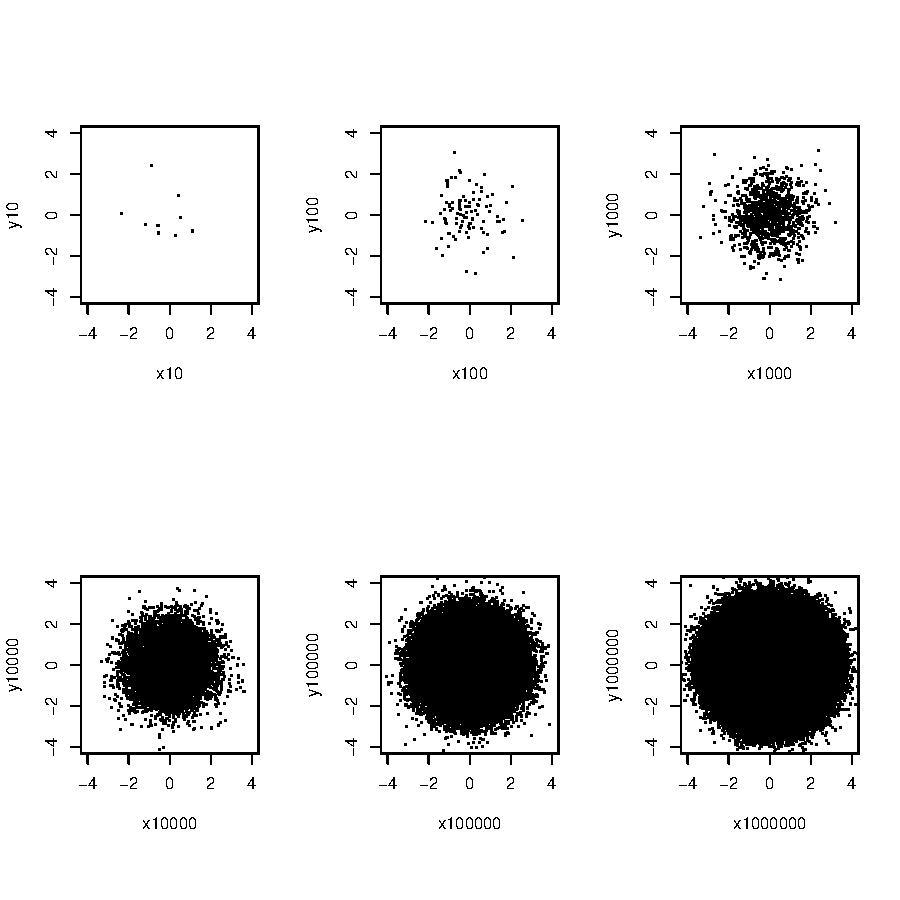
\includegraphics{lect_main-003}

{\bf Conclusion:} ``Never believe any statistics you haven't falsified yourself.'' \\
{\tiny
(\url{http://sanmateorealestateblog.com/real-estate/statistics-real-estate/never-believe-any-statistics-you-havent-falsified-yourself/})
}


\newpage


The R help page for hist indicates:
\begin{quotation}
``The generic function hist computes a histogram of the given data values.''
\end{quotation}


The R help page for the Iris data set indicates:
\begin{quotation}
``This famous (Fisher's or Anderson's) iris data set gives the measurements 
in centimeters of the variables sepal length and width and petal length and width, 
respectively, for 50 flowers from each of 3 species of iris. The species 
are {\it Iris setosa}, {\it versicolor}, and {\it virginica}.

iris is a data frame with 150 cases (rows) and 5 variables (columns) named 
Sepal.Length, Sepal.Width, Petal.Length, Petal.Width, and Species.''
\end{quotation}


\noindent
\underline{Choosing the number of classes for a histogram:} \\
As seen in the previous three examples, a bad choice for the number
of classes (nclass or breaks in the R command) in a histogram 
or the starting point of an interval and its width
can almost entirely hide the most
interesting information of the underlying data.

Several suggestions for the number of classes exist and are 
summarized in \cite{VR2002}, p.~112. We define $\mbox{range} = x_{(n)} - x_{(1)}$, 
where $n$ represents the number of observations.
\begin{itemize}
\item Sturges' formula (default in R): 
\[
\mbox{nclass} = \lceil \log_2 n + 1 \rceil, ~~~ \mbox{bin width} = \frac{\mbox{range}}{\mbox{nclass}},
\]
where $\lceil \ldots \rceil$ indicates the ceiling function.

\item Scott's 1979 formula (``scott'' in R):
\[
\mbox{bin width} = 3.5 ~ \hat{\sigma} ~ n^{-1/3}, ~~~ \mbox{nclass} = \frac{\mbox{range}}{\mbox{bin width}},
\]
where $\hat{\sigma}$ is the estimated standard deviation.

\item Freedman and Diaconis 1981 formula (``fd'' in R): 
\[
\mbox{bin width} = 2 ~ \mbox{IQR} ~ n^{-1/3}, ~~~ \mbox{nclass} = \frac{\mbox{range}}{\mbox{bin width}},
\]
where $\mbox{IQR}$ is the inter--quartile range.

\item Sometimes, the use of $\mbox{nclass} \approx \sqrt{n}$ is suggested: \\[0.2cm]
%
\url{http://www.qimacros.com/qiwizard/how-to-determine-histogram-bin-interval.htm}
suggests: {\it ``Take the square root of the number of data points and round up to 
determine the number of bins required.''} \\[0.2cm]
%
\url{http://www.moresteam.com/toolbox/t417.cfm} suggests:
{\it ``Calculate the square root of the number of data points and round to the 
nearest whole number. In the case of our height example, 
the square root of 50 is 7.07, or 7 when rounded.} \\[0.2cm]
%
\url{http://www.micquality.com/introductory_statistics/int08.htm} states: \linebreak[4]
{\it ``There are various ways of calculating the number of bins. I find that using the square root 
of the number of data values gives as good a result as the more complicated methods. 
The value is usually on the low side, but you can adjust it upwards to get convenient bin boundaries. 
Treat the calculated number of bins as a starting point, 
and adjust it as necessary to give the result you prefer.''}

\end{itemize}


\underline{\bf Example:}
%
\begin{Schunk}
\begin{Sinput}
> head(iris)
\end{Sinput}
\begin{Soutput}
  Sepal.Length Sepal.Width Petal.Length Petal.Width Species
1          5.1         3.5          1.4         0.2  setosa
2          4.9         3.0          1.4         0.2  setosa
3          4.7         3.2          1.3         0.2  setosa
4          4.6         3.1          1.5         0.2  setosa
5          5.0         3.6          1.4         0.2  setosa
6          5.4         3.9          1.7         0.4  setosa
\end{Soutput}
\begin{Sinput}
> plength <- iris[, 3]
> n <- length(plength)
> par(mfrow = c(2, 2))
> hist(plength, freq = FALSE,
+      main = "Default (Sturges) Breaks")
> hist(plength, breaks = as.integer(sqrt(n)), freq = FALSE,
+      main = "sqrt(n) Breaks")
> hist(plength, breaks = "scott", freq = FALSE,
+      main = "Scott Breaks")
> hist(plength, breaks = "fd", freq = FALSE,
+      main = "FD Breaks")
> nclass.Sturges(plength)
\end{Sinput}
\begin{Soutput}
[1] 9
\end{Soutput}
\begin{Sinput}
> sqrt(n)
\end{Sinput}
\begin{Soutput}
[1] 12.24745
\end{Soutput}
\begin{Sinput}
> nclass.scott(plength)
\end{Sinput}
\begin{Soutput}
[1] 6
\end{Soutput}
\begin{Sinput}
> nclass.FD(plength)
\end{Sinput}
\begin{Soutput}
[1] 5
\end{Soutput}
\end{Schunk}
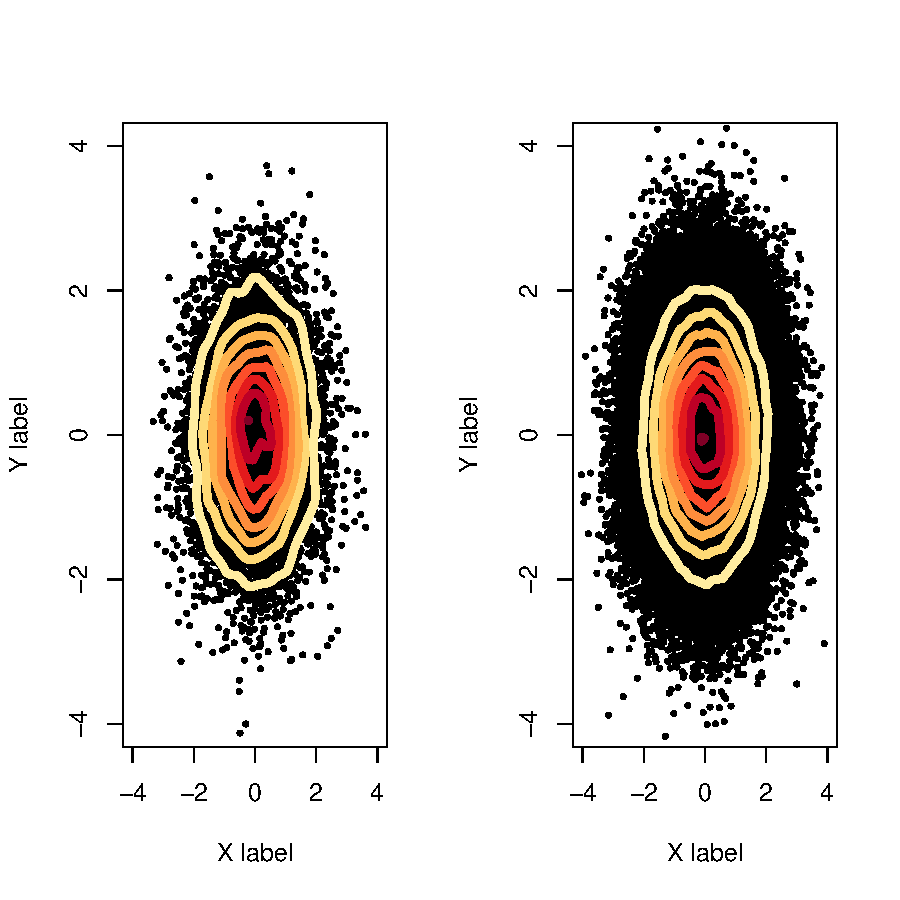
\includegraphics{lect_main-004}

Now in ggplot2:

\begin{Schunk}
\begin{Sinput}
> library(ggplot2)
> library(gridExtra)
> h1 <- ggplot(iris, aes(x = plength)) +
+   geom_histogram()
> h2 <- ggplot(iris, aes(x = plength)) +
+   geom_histogram(bins = nclass.Sturges(plength)) +
+   ggtitle("Sturges Breaks") +
+   theme(plot.title = element_text(hjust = 0.5))
> h3 <- ggplot(iris, aes(x = plength)) +
+   geom_histogram(bins = as.integer(sqrt(n))) +
+   ggtitle("sqrt(n) Breaks") +
+   theme(plot.title = element_text(hjust = 0.5))
> h4 <- ggplot(iris, aes(x = plength)) +
+   geom_histogram(bins = nclass.scott(plength)) +
+   ggtitle("Scott Breaks") +
+   theme(plot.title = element_text(hjust = 0.5))
> h5 <- ggplot(iris, aes(x = plength)) +
+   geom_histogram(bins = nclass.FD(plength)) +
+   ggtitle("FD Breaks") +
+   theme(plot.title = element_text(hjust = 0.5))
> h6 <- ggplot(iris, aes(x = plength)) +
+   geom_histogram(binwidth = 1.0, center = 0.5) +
+   ggtitle("Manually") +
+   theme(plot.title = element_text(hjust = 0.5))
> grid.arrange(h1, h2, h3, h4, h5, h6,  nrow = 2)
\end{Sinput}
\end{Schunk}
\includegraphics{lect_main-005}

Finally, how do the histograms for the three species look like?

\begin{Schunk}
\begin{Sinput}
> par(mfrow = c(2, 2))
> hist(plength, main = "all")
> hist(plength[1:50], main = "setosa")
> hist(plength[51:100], main = "versicolor")
> hist(plength[101:150], main = "virginica")
\end{Sinput}
\end{Schunk}
\includegraphics{lect_main-006}

\underline{\bf Note:} 
\begin{itemize}
\item These various methods (Sturges, Scott, FD, sqrt) provide suggestions
for the number of classes only. To enforce particular
breaks, we have to provide a vector giving the exact break points 
between the histogram cells. However, good software will use the suggestions
and then make further adjustments to obtain meaningful class breaks for a human
reader, e.g., use integers (and multiples of 5 or 10, etc.) as the boundaries.

\item Carefully check whether class intervals are left--open or right--open.
R class intervals by default are left--open whereas most readers prefer right--open
intervals. Also, check in which class interval the minimum and maximum of a data set are
included. For continuous data, there will be little differences in the 
appearance of a histogram, but for discrete data, different settings
may result in a dramatically different visual appearance of a histogram.
R provides arguments  (include.lowest and right) to adjust these options.

\item \cite{WWPJH96}, p.~30, state:
{\bf ``Since it is relatively complicated both to draw and to read
histograms with classes of different size we recommend that, as far
as possible, both tables and charts should be made with classes
of equal length.''}
\end{itemize}

\newpage 


\subsection{Averaged Shifted Histograms}


\cite{Sym2004}, p.~307, states:
\begin{quotation}
``\citet{Sc92} provides a general overview on techniques
for density estimation, including
averaged shifted histograms (ASH)
and kernel density estimators,
including possible visualization techniques via
contour surfaces,
(transparent) $\alpha$--level contours,
and contour shells.''
\end{quotation}

ASH plots were originally introduced in \citet{Sc85}.
They are created by averaging several shifted histograms
and further smoothing the result. Details are provided
in Chapter~5 of \citet{Sc92}.

ASH plots may not be easy to explain to non--statisticians,
but they may help to determine which histograms may be
closest to the underlying data.


\begin{Schunk}
\begin{Sinput}
> # Weber (2008), Set 1:
> 
> data1 <- c(.968, .982, .991, .993, .998, .999, 1.004, 1.004,
+   1.007, 1.010, 1.012, 1.015, 1.017, 1.019, 1.021,
+   1.035, 1.037, 1.037, 1.039, 1.039, 1.042, 1.042,
+   1.047, 1.053, 1.055, 1.059, 1.081, 1.107, 1.1305)
> library(ash)
> f1 <- ash1(bin1(data1, nbin = 50), 5) # compute ash estimate
\end{Sinput}
\begin{Soutput}
[1] "ash estimate nonzero outside interval ab"
\end{Soutput}
\begin{Sinput}
> par(mfrow = c(1, 3))
> hist(data1, freq = FALSE, ylim = c(0, 14)) #Default
> lines(f1 , type = "l") # line plot of estimate
> hist(data1, breaks = 0.9356 + (0:7) * 0.0325, freq = FALSE, ylim = c(0, 14)) #A
> lines(f1 , type = "l") # line plot of estimate
> hist(data1, breaks = 0.9600 + (0:7) * 0.0300, freq = FALSE, ylim = c(0, 14)) #B
> lines(f1 , type = "l") # line plot of estimate
\end{Sinput}
\end{Schunk}
\includegraphics{lect_main-007}


\begin{Schunk}
\begin{Sinput}
> # Weber (2008), Set 2:
> 
> data2 <- c(2.05, 2.27, 2.50, 2.95, 3.18, 3.41, 3.64, 3.86, 4.09, 4.32,
+   5.68, 5.91, 6.14, 6.36, 6.59, 6.82, 7.05, 7.50, 7.73, 7.95)
> f2 <- ash1(bin1(data2, nbin = 50), 5) # compute ash estimate
\end{Sinput}
\begin{Soutput}
[1] "ash estimate nonzero outside interval ab"
\end{Soutput}
\begin{Sinput}
> par(mfrow = c(2, 6))
> hist(data2, freq = FALSE, ylim = c(0, 0.25))
> lines(f2 , type ="l") # line plot of estimate
> hist(data2, breaks = 1.425 + (0:3) * 3.2075, freq = FALSE, ylim = c(0, 0.25)) #C
> lines(f2 , type = "l") # line plot of estimate
> hist(data2, breaks = -1.048 + (0:3) * 3.2075, freq = FALSE, ylim = c(0, 0.25)) #D
> lines(f2 , type = "l") # line plot of estimate
> hist(data2, breaks = 1.9767 + (0:4) * 1.9789, freq = FALSE, ylim = c(0, 0.25)) #E
> lines(f2 , type = "l") # line plot of estimate
> hist(data2, breaks = 0.1078 + (0:4) * 1.9789, freq = FALSE, ylim = c(0, 0.25)) #F
> lines(f2 , type = "l") # line plot of estimate
> hist(data2, breaks = 1.9829 + (0:5) * 1.4750, freq = FALSE, ylim = c(0, 0.25)) #G
> lines(f2 , type = "l") # line plot of estimate
> hist(data2, breaks = 0.6421 + (0:5) * 1.4750, freq = FALSE, ylim = c(0, 0.25)) #H
> lines(f2 , type = "l") # line plot of estimate
> hist(data2, breaks = 1.9619 + (0:4) * 1.9060, freq = FALSE, ylim = c(0, 0.25)) #I
> lines(f2 , type = "l") # line plot of estimate
> hist(data2, breaks = 0.8944 + (0:4) * 1.9060, freq = FALSE, ylim = c(0, 0.25)) #J
> lines(f2 , type = "l") # line plot of estimate
> hist(data2, breaks = -0.6800 + (0:4) * 2.8400, freq = FALSE, ylim = c(0, 0.25)) #K
> lines(f2 , type = "l") # line plot of estimate
> hist(data2, breaks = 1.9542 + (0:4) * 1.5229, freq = FALSE, ylim = c(0, 0.25)) #L
> lines(f2 , type = "l") # line plot of estimate
> hist(data2, breaks = 1.9619 + (0:7) * .9060, freq = FALSE, ylim = c(0, 0.25)) #New 1
> lines(f2 , type = "l") # line plot of estimate
\end{Sinput}
\end{Schunk}
\includegraphics{lect_main-008}


\newpage


\subsection{Stem--and--Leaf Plots}


The R help page for stem indicates:
\begin{quotation}
``stem produces a stem-and-leaf plot of the values in x.''
\end{quotation}


\cite{VR2002}, p.~113, further specify: 
{\it ``A stem--and--leaf plot is an enhanced histogram. The data are
divided into bins, but the `height' is replaced by the next digits in order.''}

While stem--and--leaf plots show more details than histograms, they are rarely used
in practice, in particular not for larger data sets. However, they are a useful first step
to the creation of histograms and therefore appear in many introductory statistics
textbooks, e.g.,
\cite{MMC2012}, pp.~9--12, and
\cite{Bla1998}, pp.~46--49.


\begin{Schunk}
\begin{Sinput}
> sort(plength)
\end{Sinput}
\begin{Soutput}
  [1] 1.0 1.1 1.2 1.2 1.3 1.3 1.3 1.3 1.3 1.3 1.3 1.4 1.4 1.4 1.4 1.4 1.4 1.4
 [19] 1.4 1.4 1.4 1.4 1.4 1.4 1.5 1.5 1.5 1.5 1.5 1.5 1.5 1.5 1.5 1.5 1.5 1.5
 [37] 1.5 1.6 1.6 1.6 1.6 1.6 1.6 1.6 1.7 1.7 1.7 1.7 1.9 1.9 3.0 3.3 3.3 3.5
 [55] 3.5 3.6 3.7 3.8 3.9 3.9 3.9 4.0 4.0 4.0 4.0 4.0 4.1 4.1 4.1 4.2 4.2 4.2
 [73] 4.2 4.3 4.3 4.4 4.4 4.4 4.4 4.5 4.5 4.5 4.5 4.5 4.5 4.5 4.5 4.6 4.6 4.6
 [91] 4.7 4.7 4.7 4.7 4.7 4.8 4.8 4.8 4.8 4.9 4.9 4.9 4.9 4.9 5.0 5.0 5.0 5.0
[109] 5.1 5.1 5.1 5.1 5.1 5.1 5.1 5.1 5.2 5.2 5.3 5.3 5.4 5.4 5.5 5.5 5.5 5.6
[127] 5.6 5.6 5.6 5.6 5.6 5.7 5.7 5.7 5.8 5.8 5.8 5.9 5.9 6.0 6.0 6.1 6.1 6.1
[145] 6.3 6.4 6.6 6.7 6.7 6.9
\end{Soutput}
\begin{Sinput}
> stem(plength)
\end{Sinput}
\begin{Soutput}
  The decimal point is at the |

  1 | 012233333334444444444444
  1 | 55555555555556666666777799
  2 | 
  2 | 
  3 | 033
  3 | 55678999
  4 | 000001112222334444
  4 | 5555555566677777888899999
  5 | 000011111111223344
  5 | 55566666677788899
  6 | 0011134
  6 | 6779
\end{Soutput}
\begin{Sinput}
> stem(data1)
\end{Sinput}
\begin{Soutput}
  The decimal point is 2 digit(s) to the left of the |

   96 | 8
   98 | 21389
  100 | 44702579
  102 | 157799
  104 | 227359
  106 | 
  108 | 1
  110 | 7
  112 | 1
\end{Soutput}
\begin{Sinput}
> stem(data1, scale = 2)
\end{Sinput}
\begin{Soutput}
  The decimal point is 2 digit(s) to the left of the |

   96 | 8
   97 | 
   98 | 2
   99 | 1389
  100 | 447
  101 | 02579
  102 | 1
  103 | 57799
  104 | 227
  105 | 359
  106 | 
  107 | 
  108 | 1
  109 | 
  110 | 7
  111 | 
  112 | 
  113 | 1
\end{Soutput}
\begin{Sinput}
> stem(data2)
\end{Sinput}
\begin{Soutput}
  The decimal point is at the |

  2 | 13502469
  4 | 1379
  6 | 1468157
  8 | 0
\end{Soutput}
\begin{Sinput}
> stem(data2, scale = 2)
\end{Sinput}
\begin{Soutput}
  The decimal point is at the |

  2 | 135
  3 | 02469
  4 | 13
  5 | 79
  6 | 1468
  7 | 157
  8 | 0
\end{Soutput}
\begin{Sinput}
> stem(data2, scale = 4)
\end{Sinput}
\begin{Soutput}
  The decimal point is at the |

  2 | 13
  2 | 5
  3 | 024
  3 | 69
  4 | 13
  4 | 
  5 | 
  5 | 79
  6 | 14
  6 | 68
  7 | 1
  7 | 57
  8 | 0
\end{Soutput}
\end{Schunk}


\newpage


\subsection{Boxplots (or Box--and--Whisker Plots)}


The R help page for boxplot indicates:
\begin{quotation}
``Produce box-and-whisker plot(s) of the given (grouped) values. \\[0.2cm]
range: this determines how far the plot whiskers extend out from the box. 
If range is positive, the whiskers extend to the most extreme data point which 
is no more than range times the interquartile range from the box. 
A value of zero causes the whiskers to extend to the data extremes.''
\end{quotation}

The default for range is 1.5.


\cite{VR2002}, p.~115, further specify: 
{\it ``A boxplot is a way to look at the overall shape of a set of data.
The central box shows the data between the `hinges' (roughly quartiles),
with the median represented by a line. `Whiskers' go out to the extremes
of the data, and very extreme points are shown by themselves.''}


\begin{Schunk}
\begin{Sinput}
> par(mfrow = c(2, 3))
> boxplot(plength)
> boxplot(plength, range = 0)
> boxplot(plength, range = 0.1)
> boxplot(plength ~ iris$Species)
> boxplot(plength ~ iris$Species, range = 0)
> boxplot(plength ~ iris$Species, range = 0.5)
\end{Sinput}
\end{Schunk}
\includegraphics{lect_main-010}


\begin{Schunk}
\begin{Sinput}
> par(mfrow = c(1, 2))
> boxplot(data1)
> boxplot(data2)
\end{Sinput}
\end{Schunk}
\includegraphics{lect_main-011}


\newpage


\subsection{Violin Plots}


The R help page for vioplot indicates:
\begin{quotation}
``Produce violin plot(s) of the given (grouped) values. \\[0.2cm]
A violin plot is a combination of a box plot and a kernel density plot. Specifically, 
it starts with a box plot. It then adds a rotated kernel density plot to each side of the box plot.''
\end{quotation}


\begin{Schunk}
\begin{Sinput}
> library(vioplot)
> par(mfrow = c(2, 3))
> vioplot(plength)
> vioplot(plength, range = 0)
> vioplot(plength, range = 0.1)
> vioplot(plength[iris$Species == "setosa"], 
+         plength[iris$Species == "versicolor"],
+         plength[iris$Species == "virginica"])
> vioplot(plength[iris$Species == "setosa"], 
+         plength[iris$Species == "versicolor"],
+         plength[iris$Species == "virginica"],
+         horizontal = TRUE)
> vioplot(plength[iris$Species == "setosa"], 
+         plength[iris$Species == "versicolor"],
+         plength[iris$Species == "virginica"],
+         horizontal = TRUE,
+         names = c("Setosa", "Versicolor", "Virginica"))
\end{Sinput}
\end{Schunk}
\includegraphics{lect_main-012}


\begin{Schunk}
\begin{Sinput}
> par(mfrow = c(1, 2))
> vioplot(data1)
> vioplot(data2)
\end{Sinput}
\end{Schunk}
\includegraphics{lect_main-013}


\newpage


\subsection{Letter Value Boxplots}


The R help page for LVboxplot indicates:
\begin{quotation}
``An extension of standard boxplots which draws k letter statistics. Conventional boxplots (Tukey 1977) 
are useful displays for conveying rough information about the central 50\% of the data and the 
extent of the data. \\[0.2cm]
For moderate-sized data sets (n $<$ 1000), detailed estimates of tail behavior beyond the quartiles 
may not be trustworthy [$\ldots$]. Large data sets [$\ldots$] can be expected to present a large 
number of `outliers' [$\ldots$].''
\end{quotation}


\begin{Schunk}
\begin{Sinput}
> library(lvplot)
> par(mfrow = c(2, 4))
> boxplot(plength, horizontal = TRUE)
> LVboxplot(plength)
> LVboxplot(plength, k = 1)
> LVboxplot(plength, k = 2)
> LVboxplot(plength, k = 3)
> LVboxplot(plength, k = 4)
> LVboxplot(plength, k = 5)
> LVboxplot(plength, k = 6)
\end{Sinput}
\end{Schunk}
\includegraphics{lect_main-014}


\begin{Schunk}
\begin{Sinput}
> par(mfrow = c(1, 2))
> LVboxplot(data1)
> LVboxplot(data2)
\end{Sinput}
\end{Schunk}
\includegraphics{lect_main-015}


Additional example for samples from an exponential distribution, based on LVboxplot help page:

\begin{Schunk}
\begin{Sinput}
> par(mfrow = c(4, 2), mar = c(2, 1, 3, 1))
> for (i in 1:4) {
+   x <- rexp(10^(i + 1))
+   boxplot(x, col = "grey", horizontal = TRUE,
+           ylim = c(0, 15))
+   title(paste("Exponential, n = ", length(x)))
+   LVboxplot(x, col = "grey", xlab = "",
+             xlim = c(0, 15))
+ }
\end{Sinput}
\end{Schunk}
\includegraphics{lect_main-016}


\newpage


\subsection{Dot Charts for Univariate Data}\label{DotChartsUnivariateData}


The R help page for dotchart indicates:
\begin{quotation}
``Draw a Cleveland dot plot.''
\end{quotation}


The R help page for UScereal(MASS) indicates:
\begin{quotation}
\noindent
``{\bf Nutritional and Marketing Information on US Cereals:} \\[0.2cm]
%
The UScereal data frame has 65 rows and 11 columns. The data come 
from the 1993 ASA Statistical Graphics Exposition, and are taken from 
the mandatory F\&DA food label. The data have been normalized 
here to a portion of one American cup. ''
\end{quotation}


\begin{Schunk}
\begin{Sinput}
> library(MASS)  # for cereal data
> data(UScereal)
> head(UScereal)
\end{Sinput}
\begin{Soutput}
                          mfr calories   protein      fat   sodium     fibre
100% Bran                   N 212.1212 12.121212 3.030303 393.9394 30.303030
All-Bran                    K 212.1212 12.121212 3.030303 787.8788 27.272727
All-Bran with Extra Fiber   K 100.0000  8.000000 0.000000 280.0000 28.000000
Apple Cinnamon Cheerios     G 146.6667  2.666667 2.666667 240.0000  2.000000
Apple Jacks                 K 110.0000  2.000000 0.000000 125.0000  1.000000
Basic 4                     G 173.3333  4.000000 2.666667 280.0000  2.666667
                             carbo   sugars shelf potassium vitamins
100% Bran                 15.15152 18.18182     3 848.48485 enriched
All-Bran                  21.21212 15.15151     3 969.69697 enriched
All-Bran with Extra Fiber 16.00000  0.00000     3 660.00000 enriched
Apple Cinnamon Cheerios   14.00000 13.33333     1  93.33333 enriched
Apple Jacks               11.00000 14.00000     2  30.00000 enriched
Basic 4                   24.00000 10.66667     3 133.33333 enriched
\end{Soutput}
\begin{Sinput}
> Kel.carbs <- UScereal[UScereal$mfr == "K", 7]
> Kel.carbs
\end{Sinput}
\begin{Soutput}
 [1] 21.21212 16.00000 11.00000 21.00000 13.00000 20.00000 21.00000 11.00000
 [9] 18.66667 17.50000 20.89552 26.66667 25.37313 22.38806 31.34328 20.00000
[17] 18.66667 30.00000 22.00000 12.00000 16.00000
\end{Soutput}
\begin{Sinput}
> names(Kel.carbs) <- row.names(UScereal[UScereal$mfr == "K", ])
> Kel.carbs
\end{Sinput}
\begin{Soutput}
                 All-Bran All-Bran with Extra Fiber               Apple Jacks 
                 21.21212                  16.00000                  11.00000 
              Corn Flakes                 Corn Pops        Cracklin' Oat Bran 
                 21.00000                  13.00000                  20.00000 
                  Crispix               Froot Loops            Frosted Flakes 
                 21.00000                  11.00000                  18.66667 
      Frosted Mini-Wheats             Fruitful Bran    Just Right Fruit & Nut 
                 17.50000                  20.89552                  26.66667 
     Mueslix Crispy Blend          Nut&Honey Crunch Nutri-Grain Almond-Raisin 
                 25.37313                  22.38806                  31.34328 
               Product 19               Raisin Bran            Raisin Squares 
                 20.00000                  18.66667                  30.00000 
            Rice Krispies                    Smacks                 Special K 
                 22.00000                  12.00000                  16.00000 
\end{Soutput}
\begin{Sinput}
> dotchart(Kel.carbs)
\end{Sinput}
\end{Schunk}
\includegraphics{lect_main-017}

\begin{Schunk}
\begin{Sinput}
> dotchart(sort(Kel.carbs))
\end{Sinput}
\end{Schunk}
\includegraphics{lect_main-018}

\begin{Schunk}
\begin{Sinput}
> dotchart(sort(Kel.carbs), xlim = c(10, 35), 
+   xlab = "g carbohydrates per 1 cup serving")
\end{Sinput}
\end{Schunk}
\includegraphics{lect_main-019}


Now, use the lattice package to produce similar graphs:

\begin{Schunk}
\begin{Sinput}
> library(lattice)
> dotplot(Kel.carbs)  # from lattice library
\end{Sinput}
\end{Schunk}
\includegraphics{lect_main-020}

\begin{Schunk}
\begin{Sinput}
> dotplot(sort(Kel.carbs), xlim = c(9, 36), 
+   xlab = "g carbohydrates per 1 cup serving")
\end{Sinput}
\end{Schunk}
\includegraphics{lect_main-021}


Finally, use ggplot2 to produce similar graphs:

\begin{Schunk}
\begin{Sinput}
> library(ggplot2)
> Kel.carbsdf <- data.frame(Brand = as.factor(names(Kel.carbs)), Carbs = Kel.carbs)
> Kel.carbsdf 
\end{Sinput}
\begin{Soutput}
                                              Brand    Carbs
All-Bran                                   All-Bran 21.21212
All-Bran with Extra Fiber All-Bran with Extra Fiber 16.00000
Apple Jacks                             Apple Jacks 11.00000
Corn Flakes                             Corn Flakes 21.00000
Corn Pops                                 Corn Pops 13.00000
Cracklin' Oat Bran               Cracklin' Oat Bran 20.00000
Crispix                                     Crispix 21.00000
Froot Loops                             Froot Loops 11.00000
Frosted Flakes                       Frosted Flakes 18.66667
Frosted Mini-Wheats             Frosted Mini-Wheats 17.50000
Fruitful Bran                         Fruitful Bran 20.89552
Just Right Fruit & Nut       Just Right Fruit & Nut 26.66667
Mueslix Crispy Blend           Mueslix Crispy Blend 25.37313
Nut&Honey Crunch                   Nut&Honey Crunch 22.38806
Nutri-Grain Almond-Raisin Nutri-Grain Almond-Raisin 31.34328
Product 19                               Product 19 20.00000
Raisin Bran                             Raisin Bran 18.66667
Raisin Squares                       Raisin Squares 30.00000
Rice Krispies                         Rice Krispies 22.00000
Smacks                                       Smacks 12.00000
Special K                                 Special K 16.00000
\end{Soutput}
\begin{Sinput}
> ggplot(Kel.carbsdf, aes(x = Carbs, y = Brand)) +
+   geom_point()
\end{Sinput}
\end{Schunk}
\includegraphics{lect_main-022}


\begin{Schunk}
\begin{Sinput}
> # reorder by carbs
> Kel.carbsdf$Brand <- factor(Kel.carbsdf$Brand,
+                             levels = Kel.carbsdf$Brand[order(Kel.carbsdf$Carbs)])
> Kel.carbsdf$Brand
\end{Sinput}
\begin{Soutput}
 [1] All-Bran                  All-Bran with Extra Fiber
 [3] Apple Jacks               Corn Flakes              
 [5] Corn Pops                 Cracklin' Oat Bran       
 [7] Crispix                   Froot Loops              
 [9] Frosted Flakes            Frosted Mini-Wheats      
[11] Fruitful Bran             Just Right Fruit & Nut   
[13] Mueslix Crispy Blend      Nut&Honey Crunch         
[15] Nutri-Grain Almond-Raisin Product 19               
[17] Raisin Bran               Raisin Squares           
[19] Rice Krispies             Smacks                   
[21] Special K                
21 Levels: Apple Jacks Froot Loops Smacks ... Nutri-Grain Almond-Raisin
\end{Soutput}
\begin{Sinput}
> ggplot(Kel.carbsdf, aes(x = Carbs, y = Brand)) +
+   geom_point()
\end{Sinput}
\end{Schunk}
\includegraphics{lect_main-023}


The web site at \url{https://www.r-bloggers.com/revisiting-clevelands-the-elements-of-graphing-data-in-ggplot2/}
provides some useful suggestions how to further improve the appearance of these graphs:

\begin{Schunk}
\begin{Sinput}
> # make some further adjustments to the appearance of the grid
> ggplot(Kel.carbsdf, aes(x = Carbs, y = Brand)) +
+   geom_point() +
+   theme( 
+     # remove the vertical grid lines
+     panel.grid.major.x = element_blank(),
+     panel.grid.minor.x = element_blank(),
+     # explicitly set the horizontal grid lines
+     panel.grid.major.y = element_line(linetype = 3, color = "darkgray"),
+     axis.text.y = element_text(size = rel(0.8))) +
+   xlab("Carbs (g carbohydrates per 1 cup serving)")
> # ineractive version
> library(plotly)
> ggplotly()
\end{Sinput}
\end{Schunk}
\includegraphics{lect_main-024}


\newpage


The R help page for barley in the lattice package indicates:
\begin{quotation}
\noindent
``{\bf Yield data from a Minnesota barley trial:} \\[0.2cm]
%
Total yield in bushels per acre for 10 varieties at 6 sites in each of two years.''
\end{quotation}


\begin{Schunk}
\begin{Sinput}
> library(lattice)  # for barley data
> data(barley)
> head(barley)
\end{Sinput}
\begin{Soutput}
     yield   variety year            site
1 27.00000 Manchuria 1931 University Farm
2 48.86667 Manchuria 1931          Waseca
3 27.43334 Manchuria 1931          Morris
4 39.93333 Manchuria 1931       Crookston
5 32.96667 Manchuria 1931    Grand Rapids
6 28.96667 Manchuria 1931          Duluth
\end{Soutput}
\begin{Sinput}
> dotplot(variety ~ yield | site, data = barley, groups = year,
+   key = simpleKey(levels(barley$year), space = "right"),
+   xlab = "Barley Yield (bushels/acre)",
+   aspect = 0.5, layout = c(1, 6), ylab = NULL)
\end{Sinput}
\end{Schunk}
\includegraphics{lect_main-025}

\begin{Schunk}
\begin{Sinput}
> levels(barley$site)
\end{Sinput}
\begin{Soutput}
[1] "Grand Rapids"    "Duluth"          "University Farm" "Morris"         
[5] "Crookston"       "Waseca"         
\end{Soutput}
\begin{Sinput}
> # alphabetical sorting of sites (top to bottom)
> dotplot(variety ~ yield | site, data = barley, groups = year, 
+   key = simpleKey(levels(barley$year), space = "right"), 
+   xlab = "Barley Yield (bushels/acre)", 
+   aspect = 0.5, layout = c(1, 6), ylab = NULL,
+   index.cond = list(c(6, 3, 4, 1, 2, 5))) 
\end{Sinput}
\end{Schunk}
\includegraphics{lect_main-026}


\noindent
\underline{\bf Question:} \\
What is the most striking (unusual) feature in these plots? 
Look carefully!


\newpage


\subsection{Kernel Density Plots for Univariate Data (with Rug Plot)}


The R help page for density indicates:
\begin{quotation}
\noindent
``{\bf Kernel Density Estimation:} \\[0.2cm]
The (S3) generic function density computes kernel density estimates. 
Its default method does so with the given kernel and bandwidth for univariate observations. 
[$\ldots$] \\
bw: the smoothing bandwidth to be used. The kernels are scaled such that this is the 
standard deviation of the smoothing kernel. (Note this differs from the reference books 
cited below, and from S--PLUS.) \\
bw can also be a character string giving a rule to choose the bandwidth. See bw.nrd. \\
The specified (or computed) value of bw is multiplied by adjust.''
\end{quotation}


The R help page for rug indicates:
\begin{quotation}
``Adds a rug representation (1-d plot) of the data to the plot.''
\end{quotation}

\cite{CH93}, p.~548, further specify: {\it ``rug: [$\ldots$]
a univariate histogram or rugplot is displayed along the base 
of each plot, showing the occurrence of each $x$--value; ties are
broken by jittering.''}


\begin{Schunk}
\begin{Sinput}
> par(mfrow = c(3, 2))
> plot(density(plength), xlim = c(-1, 9))                # default nrd0 bw
> rug(plength, ticksize = 0.05)
> plot(density(plength, bw = "nrd"), xlim = c(-1, 9))    # normal reference rule bw
> rug(plength, ticksize = 0.05)
> plot(density(plength, bw = "ucv"), xlim = c(-1, 9))    
>                                    # unbiased cross-validation rule bw
> rug(plength, ticksize = 0.05)
> plot(density(plength, bw = "bcv"), xlim = c(-1, 9))    
>                                    # biased cross-validation rule bw
> rug(plength, ticksize = 0.05)
> plot(density(plength, bw = "SJ-ste"), xlim = c(-1, 9)) 
>                                    # Sheather-Jones ("solve-the-equation") bw
> rug(plength, ticksize = 0.05)
> plot(density(plength, bw = "SJ-dpi"), xlim = c(-1, 9)) 
>                                    # Sheather-Jones ("direct plug-in") bw
> rug(plength, ticksize = 0.05)
\end{Sinput}
\end{Schunk}
\includegraphics{lect_main-027}


\begin{Schunk}
\begin{Sinput}
> par(mfrow = c(3, 2))
> plot(density(plength), xlim = c(-1, 9))
> plot(density(plength, adjust = 1/2), xlim = c(-1, 9))  #adjust default bandwidth
> plot(density(plength, adjust = 1/4), xlim = c(-1, 9))
> plot(density(plength, adjust = 1/8), xlim = c(-1, 9))
> plot(density(plength, adjust = 2), xlim = c(-1, 9))
> plot(density(plength, adjust = 4), xlim = c(-1, 9))
\end{Sinput}
\end{Schunk}
\includegraphics{lect_main-028}


Now, use the lattice package and produce similar graphics:
\begin{Schunk}
\begin{Sinput}
> library(lattice)
> dp1 <- densityplot(plength)  # lattice, takes all parameters from density (above)
> dp2 <- densityplot(plength, n = 512)
> dp3 <- densityplot(plength, n = 512, bw = "SJ")
> # arrange the three plots vertically
> print(dp1, position = c(0, 0, 1, 0.33), more = TRUE)
> print(dp2, position = c(0, 0.33, 1, 0.66), more = TRUE)
> print(dp3, position = c(0, 0.66, 1, 0.99))
\end{Sinput}
\end{Schunk}
\includegraphics{lect_main-029}

In {\it densityplot}, n is the ``number of points at which density is to be evaluated''
and the default is 50.


Now in ggplot2. The web page 
\url{https://stackoverflow.com/questions/32468772/histogram-with-a-jittery-rug}
provided some suggestions how to add the jittered rug.


\begin{Schunk}
\begin{Sinput}
> library(ggplot2)
> library(gridExtra)
> h1 <- ggplot(iris, aes(x = plength)) +
+   xlim(-1, 9) +
+   geom_histogram(binwidth = 0.5, center = 0.25) +
+   ggtitle("Histogram") +
+   theme(plot.title = element_text(hjust = 0.5))
> h2 <- ggplot(iris, aes(x = plength)) +
+   xlim(-1, 9) +
+   geom_histogram(aes(y = ..density..), binwidth = 0.5, center = 0.25) +
+   ggtitle("Histogram (Density Scale)") +
+   theme(plot.title = element_text(hjust = 0.5))
> h3 <- ggplot(iris, aes(x = plength)) +
+   xlim(-1, 9) +
+   geom_histogram(aes(y = ..density..), binwidth = 0.5, center = 0.25) +
+   ggtitle("Histogram Density (Default)") +
+   theme(plot.title = element_text(hjust = 0.5)) +
+   geom_density()
> h4 <- ggplot(iris, aes(x = plength)) +
+   xlim(-1, 9) +
+   geom_histogram(aes(y = ..density..), binwidth = 0.5, center = 0.25) +
+   ggtitle("Histogram Density (SJ-ste)") +
+   theme(plot.title = element_text(hjust = 0.5)) +
+   geom_density(bw = "SJ-ste", col = "red")
> h5 <- ggplot(iris, aes(x = plength)) +
+   xlim(-1, 9) +
+   ylim(0, 0.6) +
+   geom_histogram(aes(y = ..density..), binwidth = 0.5, center = 0.25) +
+   ggtitle("Histogram & Density & Rug") +
+   theme(plot.title = element_text(hjust = 0.5)) +
+   geom_density(bw = "SJ-ste", col = "red") +
+   geom_rug()
> h6 <- ggplot(iris, aes(x = plength)) +
+   xlim(-1, 9) +
+   ylim(0, 0.6) +
+   geom_histogram(aes(y = ..density..), binwidth = 0.5, center = 0.25) +
+   ggtitle("Histogram & Density & Rug (Final)") +
+   theme(plot.title = element_text(hjust = 0.5)) +
+   geom_density(bw = "SJ-ste", col = "red") +
+   geom_rug(sides = "b", aes(y = 0.4), position = "jitter", col = "blue")
> grid.arrange(h1, h2, h3, h4, h5, h6, nrow = 2)
\end{Sinput}
\end{Schunk}
\includegraphics{lect_main-030}


\newpage


\subsection{Quantile--Quantile Plots (Q--Q Plots)}


One of the best ways to compare the distribution of a sample $\ux$ of size $n$
with an assumed theoretical distribution $F$ is to use a 
Quantile--Quantile Plot (Q--Q Plot). In such a plot, we plot
the pairs of points
\[
\left( F^{-1} \left( \frac{i - 0.5}{n} \right), x_{(i)} \right), 
~~ i = 1, \ldots, n.
\]


\noindent
\underline{\bf Example 1:} \\
Convergence of a $t$ distribution with $df$ degrees of freedom
towards a normal distribution.

\begin{Schunk}
\begin{Sinput}
> # set seed of random number generator to be able to reproduce results
> set.seed(2) 
> par(mfrow = c(3, 2))
> tdf1 <- rt(100, df = 1)
> qqnorm(tdf1)
> qqline(tdf1)
> tdf2 <- rt(100, df = 2)
> qqnorm(tdf2)
> qqline(tdf2)
> tdf5 <- rt(100, df = 5)
> qqnorm(tdf5)
> qqline(tdf5)
> tdf10 <- rt(100, df = 10)
> qqnorm(tdf10)
> qqline(tdf10)
> tdf20 <- rt(100, df = 20)
> qqnorm(tdf20)
> qqline(tdf20)
> tdf30 <- rt(100, df = 30)
> qqnorm(tdf30)
> qqline(tdf30)
\end{Sinput}
\end{Schunk}
\includegraphics{lect_main-031}


\noindent
\underline{\bf Note:} \\
The closer the points from the sample fall to a straight line,
the closer the sample distribution and the theoretical distribution
are related. However, here, the greater spread of the extreme quantiles
for the sample (for $df = 1, 2, 5, 10, 20$)
is an indicator of a long--tailed distribution.


A quick glance at Q--Q--plots via ggplot2, with additional suggestions from
\url{http://ggplot2.tidyverse.org/reference/geom_qq.html} and
\url{https://gist.github.com/slowkow/9041570}.

\begin{Schunk}
\begin{Sinput}
> library(ggplot2)
> library(gridExtra)
> tdf1df <- data.frame(y = tdf1)
> q1 <- ggplot(tdf1df, aes(sample = y)) +
+   stat_qq() +
+   geom_abline(intercept = 0, slope = 1, alpha = 0.5)
> tdf30df <- data.frame(y = tdf30)
> q30 <- ggplot(tdf30df, aes(sample = y)) +
+   stat_qq() +
+   geom_abline(intercept = 0, slope = 1, alpha = 0.5)
> grid.arrange(q1, q30, nrow = 1)
\end{Sinput}
\end{Schunk}
\includegraphics{lect_main-032}


\noindent
\underline{\bf Example 2:} \\
Recall: What is the relationship between exponential
distributions and Gamma distributions? Verify this graphically!

\begin{Schunk}
\begin{Sinput}
> par(mfrow = c(3, 2))
> set.seed(4) 
> exp1 <- rexp(100, rate = 1)
> plot(qgamma(ppoints(exp1), 1, 1), sort(exp1))
> abline(0, 1)
> exp2 <- rexp(100, rate = 2)
> plot(qgamma(ppoints(exp2), 1, 2), sort(exp2))
> abline(0, 1)
> exp5 <- rexp(100, rate = 5)
> plot(qgamma(ppoints(exp5), 1, 5), sort(exp5))
> abline(0, 1)
> exp10 <- rexp(100, rate = 10)
> plot(qgamma(ppoints(exp10), 1, 10), sort(exp10))
> abline(0, 1)
> # Some major misspecifications
> 
> # a) Swapping shape and rate parameters
> plot(qgamma(ppoints(exp2), 2, 1), sort(exp2))
> abline(0, 1)
> # b) Using 1/rate instead
> plot(qgamma(ppoints(exp2), 1, 1/2), sort(exp2))
> abline(0, 1)
\end{Sinput}
\end{Schunk}
\includegraphics{lect_main-033}


\underline{\bf Example 3:} \\
Compare iris plength sample data with an underlying assumed normal distribution.
For which of the species is the assumption of normality justified?

\begin{Schunk}
\begin{Sinput}
> par(mfrow = c(2, 2))
> qqnorm(plength)
> qqnorm(plength[1:50])
> qqnorm(plength[51:100])
> qqnorm(plength[101:150])
\end{Sinput}
\end{Schunk}
\includegraphics{lect_main-034}


\newpage


\subsection{Empirical Cumulative Distribution Functions (ECDFs)}


Recall from Stat 6720: \\

\underline{Definition 7.1.3:} \\
Let $X_1, \ldots, X_n$ be a sample of size $n$ from a population with
distribution $F$. The function
\[
\hat{F_n} (x) = \frac{1}{n} \displaystyle\sum_{i=1}^n
  I_{(-\infty, x]} (X_i)
\]
is called 
{\bf empirical cumulative distribution function} 
({\bf empirical cdf, ECDF}).
$\qedsymb$ \\


\underline{Theorem 7.1.7:}
{\bf Glivenko--Cantelli Theorem}\index{Glivenko--Cantelli Theorem} \\
%
$\hat{F_n} (x)$ converges uniformly to $F(x)$, i.e., it holds
for all $\epsilon > 0$ that
\[
\displaystyle\lim_{n \rightarrow \infty}
  P(\sup_{-\infty < x < \infty} \mid \hat{F_n} (x) - F(x) \mid >
   \epsilon) = 0.
\]
$\qedsymb$


Verify this theorem for samples from a normal distribution:

\begin{Schunk}
\begin{Sinput}
> par(mfrow = c(2, 2))
> set.seed(1234) 
> xvals <- seq(-4, 4, 0.01)
> norm10 <- rnorm(10)
> plot(ecdf(norm10), xlim = c(-4, 4))
> lines(xvals, pnorm(xvals))
> norm25 <- rnorm(25)
> plot(ecdf(norm25), xlim = c(-4, 4))
> lines(xvals, pnorm(xvals))
> norm100 <- rnorm(100)
> plot(ecdf(norm100), xlim = c(-4, 4))
> lines(xvals, pnorm(xvals))
> norm1000 <- rnorm(1000)
> plot(ecdf(norm1000), xlim = c(-4, 4))
> lines(xvals, pnorm(xvals))
\end{Sinput}
\end{Schunk}
\includegraphics{lect_main-035}


\begin{Schunk}
\begin{Sinput}
> # Animation
> par(mfrow = c(1, 1))
> xvals <- seq(-4, 4, 0.01)
> pnormxvals <- pnorm(xvals)
> normgrow <- NULL
> for (i in 1:150) {
+   normgrow <- c(normgrow, rnorm(1))
+   plot(ecdf(normgrow), xlim = c(-4, 4), main = length(normgrow))
+   lines(xvals, pnormxvals, col = "red")
+   Sys.sleep(0.1)
+ }
\end{Sinput}
\end{Schunk}


\noindent
\underline{\bf Example:} \\
And here the ECDF for iris plength.

\begin{Schunk}
\begin{Sinput}
> plot(ecdf(plength)) 
\end{Sinput}
\end{Schunk}
\includegraphics{lect_main-037}


\newpage


\subsection{Graphics and Small Sample Sizes}


\centerline{\Large \bf Worksheet}~\\

\centerline{\hfill {\large \bf Your Name:} \underline{\hspace*{5cm}}}


\underline{\bf Question:} \\

The data shown in these four histograms originate from which 
distribution?

%\begin{figure}[h]
%\centering{\includegraphics[width=3.5in]{Scans//Chapter5_unknown_hist.jpg}}
%\caption{\label{Chapter5_unknown_hist}
%Histograms for data from four unknown distributions.
%}
%\end{figure}

The corresponding distributions are: \\[0.5cm]
%
Upper left: \underline{\hspace*{3cm}} \\[0.2cm]
Upper right: \underline{\hspace*{3cm}} \\[0.2cm]
Lower left: \underline{\hspace*{3cm}} \\[0.2cm]
Lower right: \underline{\hspace*{3cm}}


\newpage


\centerline{\Large \bf Worksheet}~\\

\centerline{\hfill {\large \bf Your Name:} \underline{\hspace*{5cm}}}


\underline{\bf Question:} \\

Do the data shown in these four qqplots follow a normal
distribution?

%\begin{figure}[h]
%\centering{\includegraphics[width=3.8in]{Scans//Chapter5_unknown_qqplot.jpg}}
%\caption{\label{Chapter5_unknown_qqplot}
%Normal QQplots for data from four unknown distributions.
%}
%\end{figure}

So, does a particular qqplot suggest that the data 
originate from a normal distribution? Circle your answer: \\[0.5cm]
%
Upper left: {\bf ~~ yes ~~ / ~~ no} \\[0.2cm]
Upper right: {\bf ~~ yes ~~ / ~~ no} \\[0.2cm]
Lower left: {\bf ~~ yes ~~ / ~~ no} \\[0.2cm]
Lower right: {\bf ~~ yes ~~ / ~~ no}


\newpage


\if\jsprivatechfive 1

\underline{\bf Answers:}

The following R code was used to create the figures shown on the previous
two pages:

\begin{Schunk}
\begin{Sinput}
> set.seed(1234)
> jpeg("Chapter5_unknown_hist.jpg")
> par(mfrow = c(2, 2))
> xvect1 <- NULL
> for (i in 1:4) {
+   x <- rnorm(10)
+   xvect1 <- c(xvect1, x)
+   hist(x, main = "Unknown Distribution",
+     xlab = "x-values")
+ }
> dev.off()
\end{Sinput}
\begin{Soutput}
pdf 
  2 
\end{Soutput}
\end{Schunk}


\begin{Schunk}
\begin{Sinput}
> set.seed(1234)
> jpeg("Chapter5_unknown_qqplot.jpg")
> par(mfrow = c(2, 2))
> xvect2 <- NULL
> for (i in 1:4) {
+   x <- rnorm(10)
+   xvect2 <- c(xvect2, x)
+   qqnorm(x, main = "Unknown Distribution",
+     xlab = "Normal Quantiles")
+ }
> dev.off()
\end{Sinput}
\begin{Soutput}
pdf 
  2 
\end{Soutput}
\end{Schunk}


\newpage


When we jointly plot all 40 observations, we start
to see that the underlying distribution indeed is a
normal distribution. In fact, all eight plots 
on the previous two pages show
10 samples each drawn from the standard normal distribution!

\begin{Schunk}
\begin{Sinput}
> # Plot all data combined
> 
> par(mfrow = c(1, 1))
> hist(xvect1)
\end{Sinput}
\end{Schunk}
\includegraphics{lect_main-040}


\begin{Schunk}
\begin{Sinput}
> par(mfrow = c(1, 1))
> qqnorm(xvect2)
\end{Sinput}
\end{Schunk}
\includegraphics{lect_main-041}


\else
{\bf Additional details will be provided after class.}
\fi


\newpage


\subsection{Further Reading}

Additional sources for Trellis Graphics are:

\begin{itemize}
\item Trellis dipsplays at Bell Labs (in S/S--Plus; needs some updates for modern R):
\url{http://ect.bell-labs.com/sl/project/trellis/}

\item \cite{Mu2006}, Chapter 4:
\url{https://www.stat.auckland.ac.nz/~paul/RGraphics/chapter4.pdf}

\item William G. Jacoby's web page on dot plots:
\url{http://polisci.msu.edu/jacoby/research/statgrph/tpm/sdlist.html}

\end{itemize}


~\\[-0.5cm]

%\begin{figure}[ht]
%\centering{\includegraphics[height=4in]{Scans//Cartoonstock_SalesChart.jpg}}
%\caption{\label{Cartoonstock_SalesChart}
%url{http://www.cartoonstock.com/blowup_stock.asp?imageref=forn395&artist=Fran&topic=statistics+},
%Cartoon.
%}
%\end{figure}


\newpage


%\SweaveInput{lect_chapter6.Rnw}
%\SweaveInput{lect_chapter1.Rnw}
%
%\SweaveInput{lect_chapter2.Rnw}
%\SweaveInput{lect_chapter3.Rnw}
%\SweaveInput{lect_chapter9.Rnw}
%\SweaveInput{lect_chapter7.Rnw}
%\SweaveInput{lect_chapter8.Rnw}
%\SweaveInput{lect_chapter10.Rnw}


\setcounter{page}{1}
\addcontentsline{toc}{section}{References}

\bibliography{references}


\vspace*{1cm}

\centering{\bf \LARGE --- THE END ---}~\\[1cm]

%\begin{figure}[ht]
%\centering{\includegraphics[height=3in]{Scans//Cartoonstock_FallingArrow.jpg}}
%\caption{\label{Cartoonstock_FallingArrow}
%\url{http://www.cartoonstock.com/blowup_stock.asp?imageref=vsh0184&artist=Shirvanian,+Vahan&topic=statistics+}, 
%Cartoon.
%}
%\end{figure}


\end{document}

